\section{Experiments}
\begin{frame}{Robotcar dataset}
	\begin{figure}[t]
		\centering
		
		\only<1>{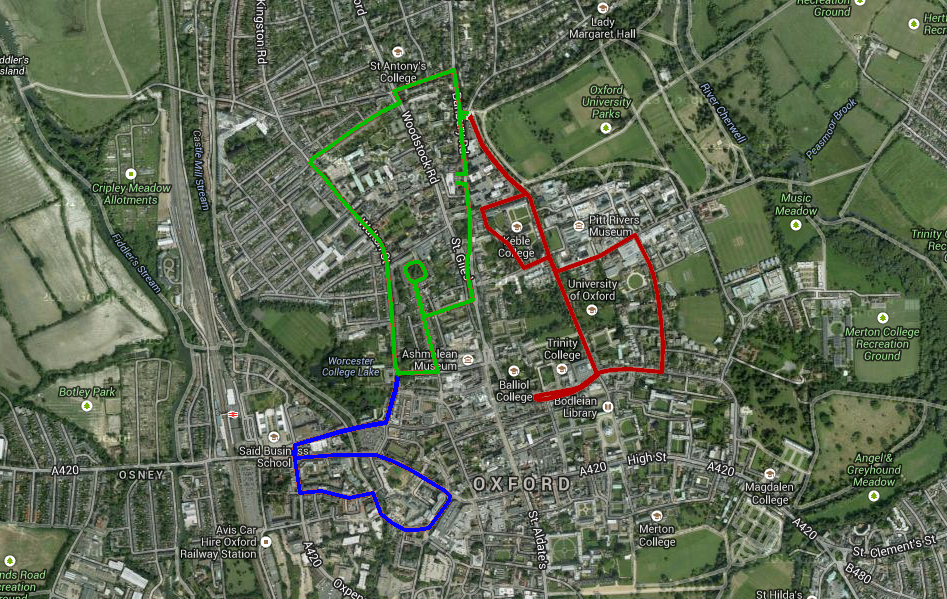
\includegraphics[width=0.8\linewidth]{images/map/map.png}  }
		\only<2>{
		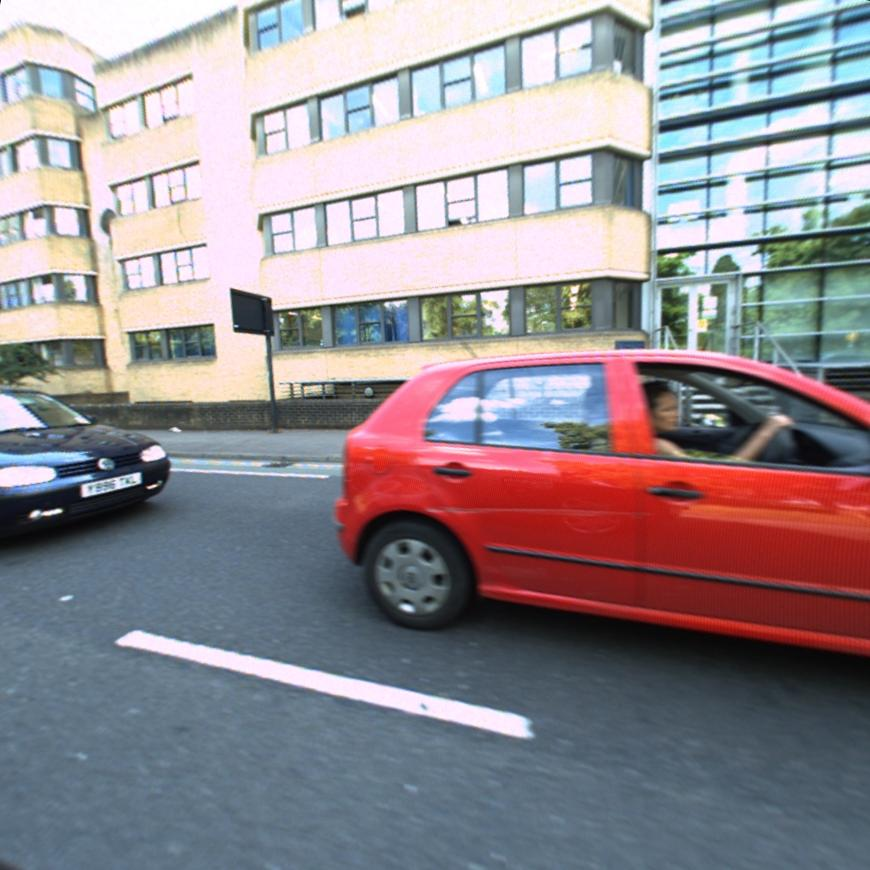
\includegraphics[width=0.19\linewidth]{images/ex_query/query0.jpg}\hfill
		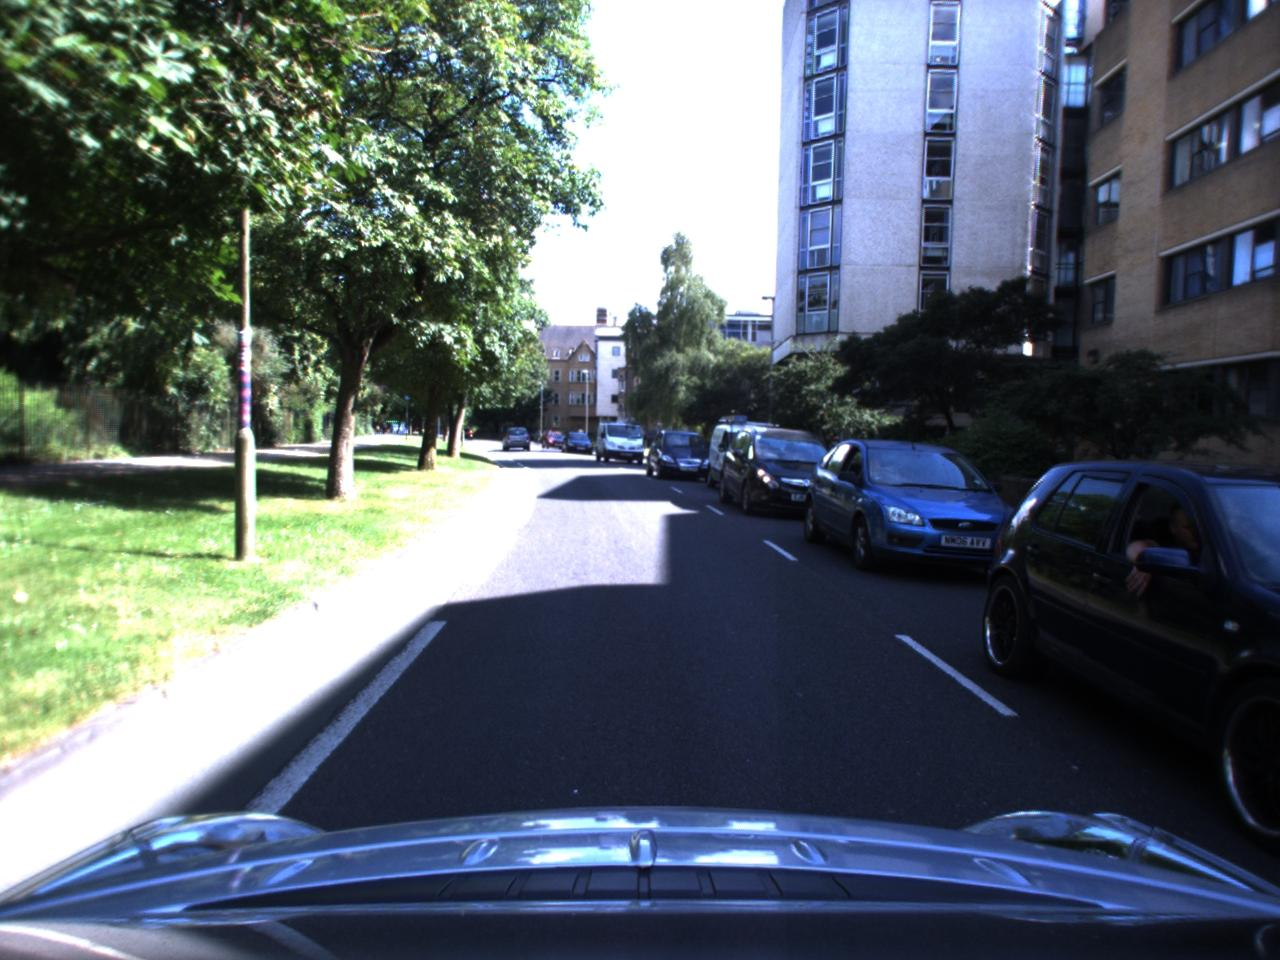
\includegraphics[width=0.23\linewidth]{images/ex_query/query1.jpg}\hfill
		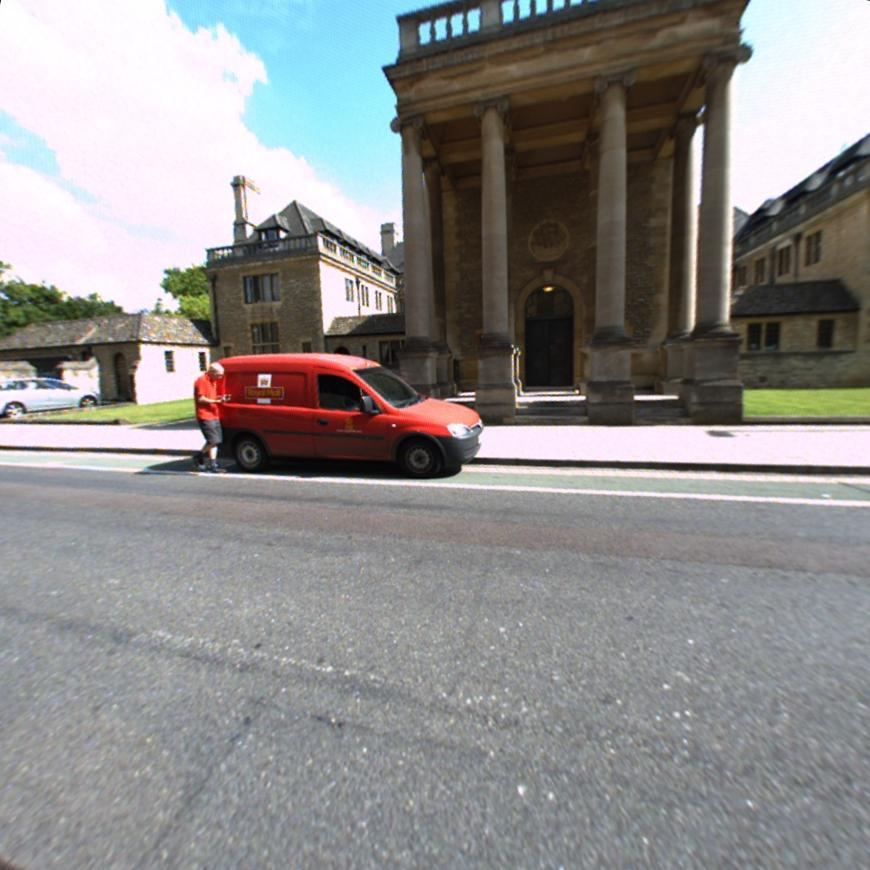
\includegraphics[width=0.19\linewidth]{images/ex_query/query2.jpg}\hfill
		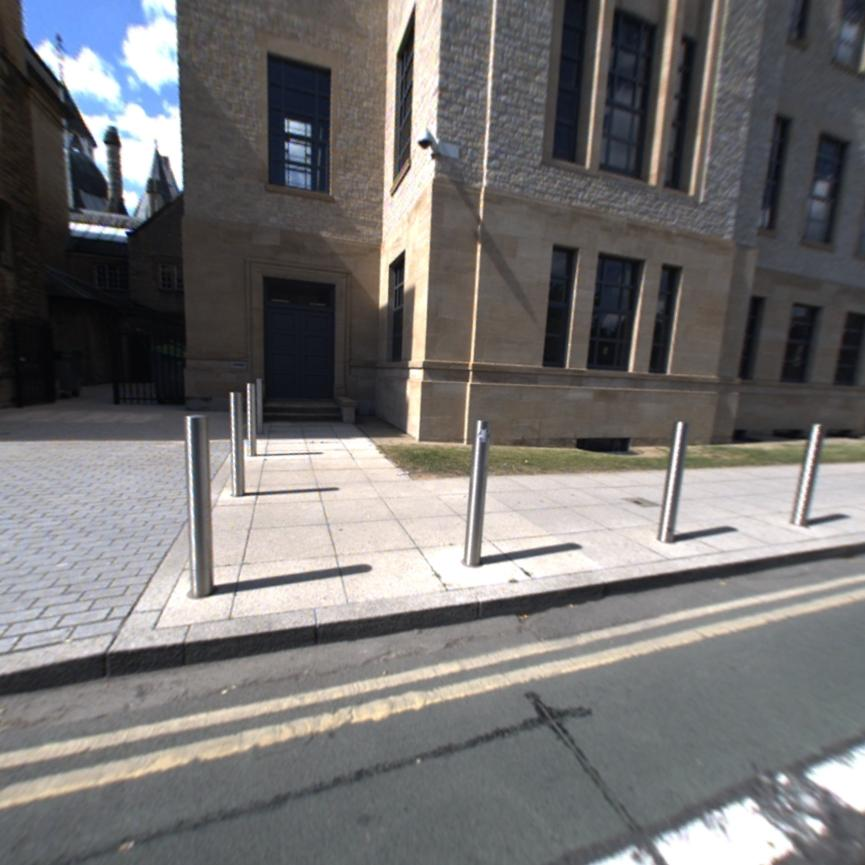
\includegraphics[width=0.19\linewidth]{images/ex_query/query3.jpg}\hfill
		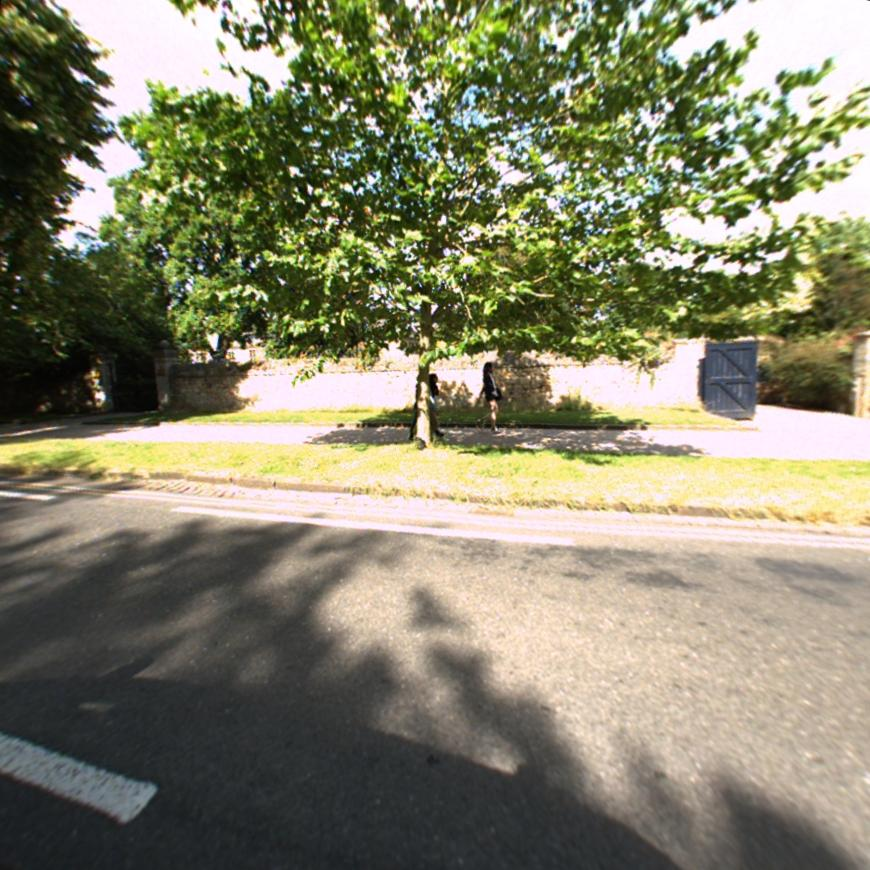
\includegraphics[width=0.19\linewidth]{images/ex_query/query4.jpg}
			
		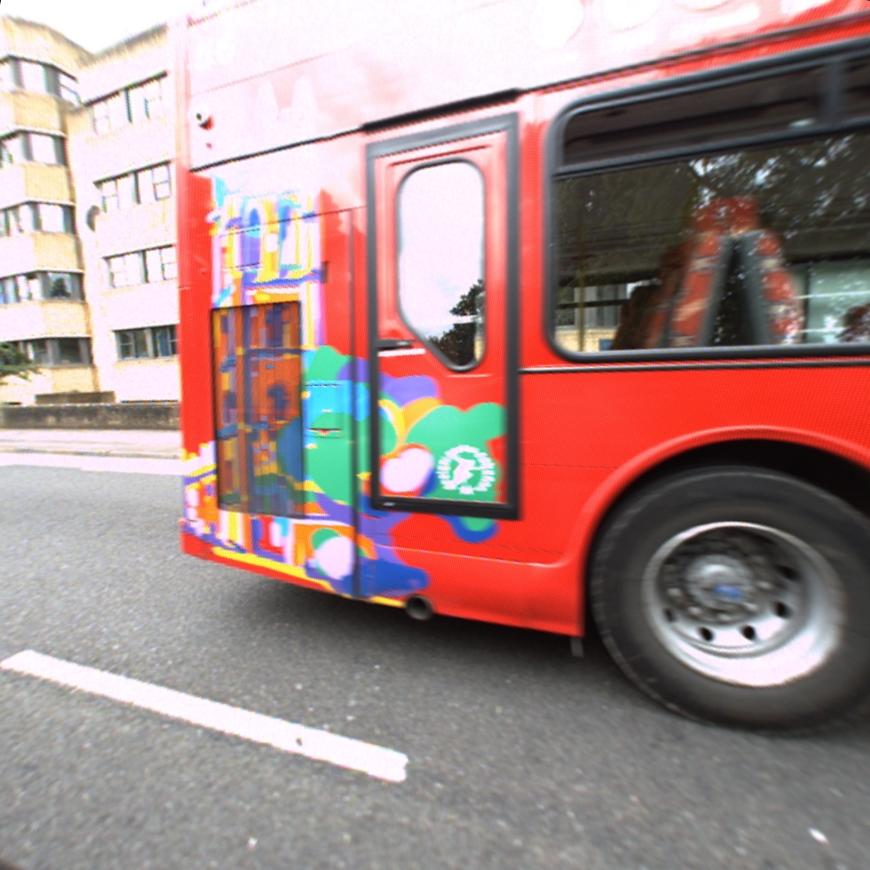
\includegraphics[width=0.19\linewidth]{images/ex_query/dataset0.jpg}\hfill
		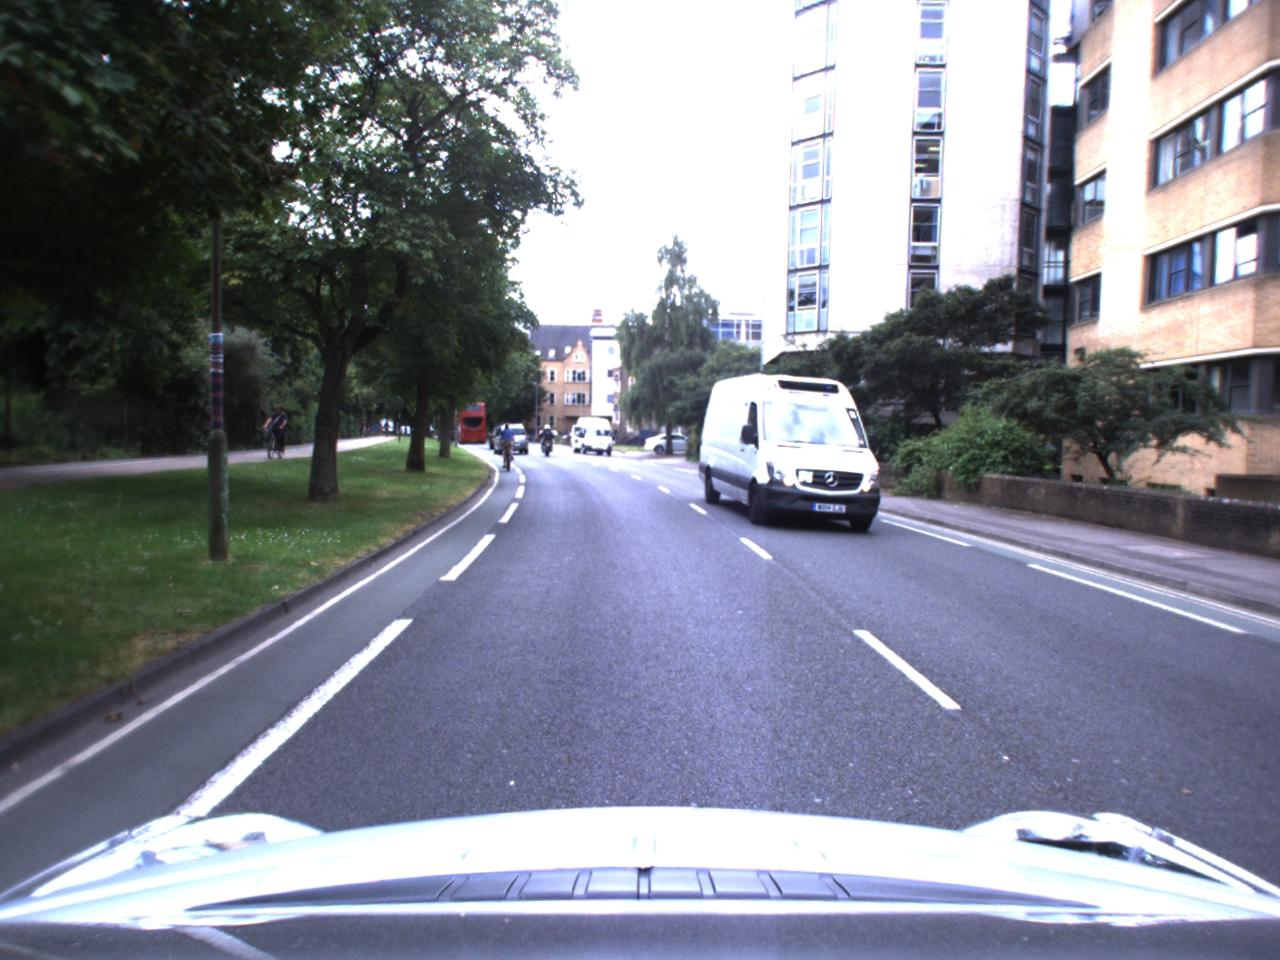
\includegraphics[width=0.23\linewidth]{images/ex_query/dataset1.jpg}\hfill
		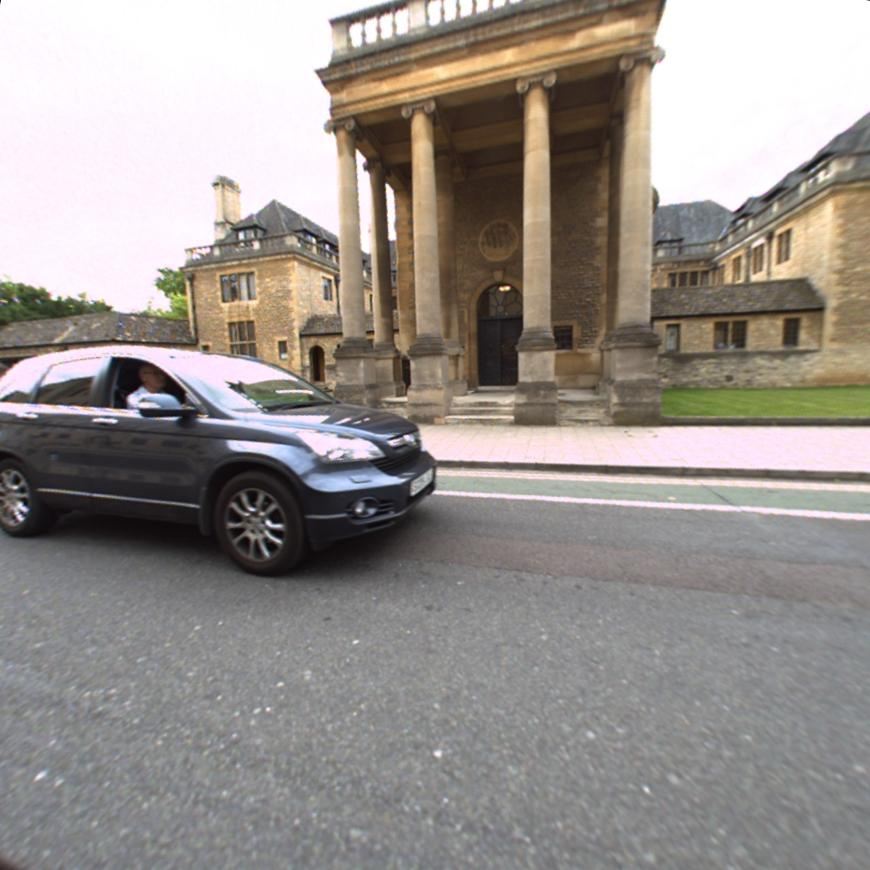
\includegraphics[width=0.19\linewidth]{images/ex_query/dataset2.jpg}\hfill
		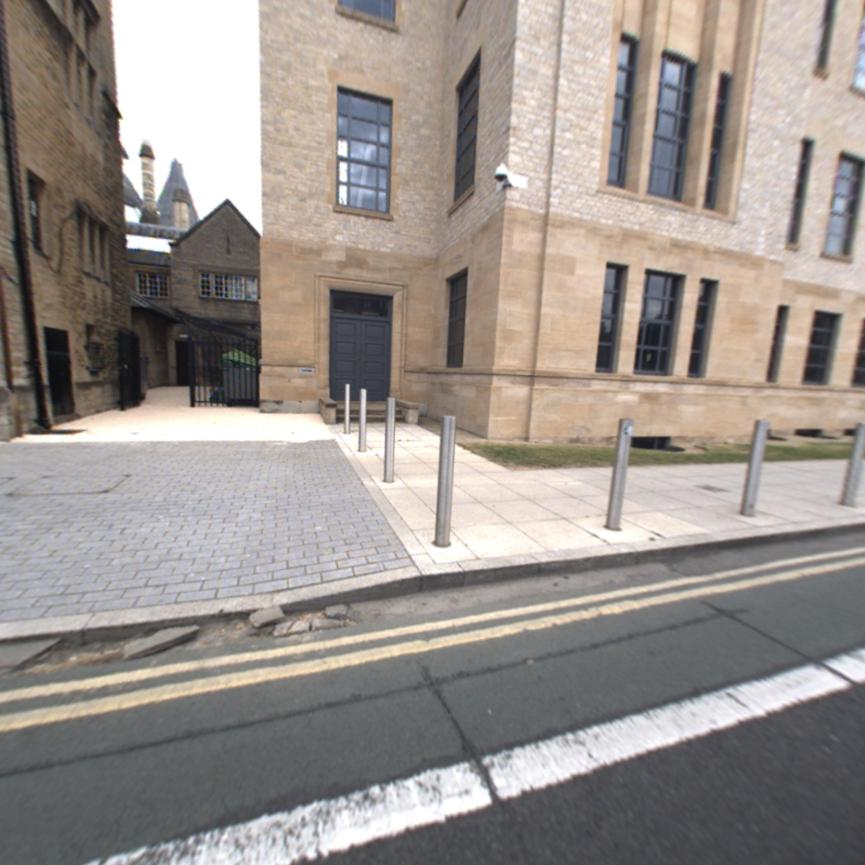
\includegraphics[width=0.19\linewidth]{images/ex_query/dataset3.jpg}\hfill
		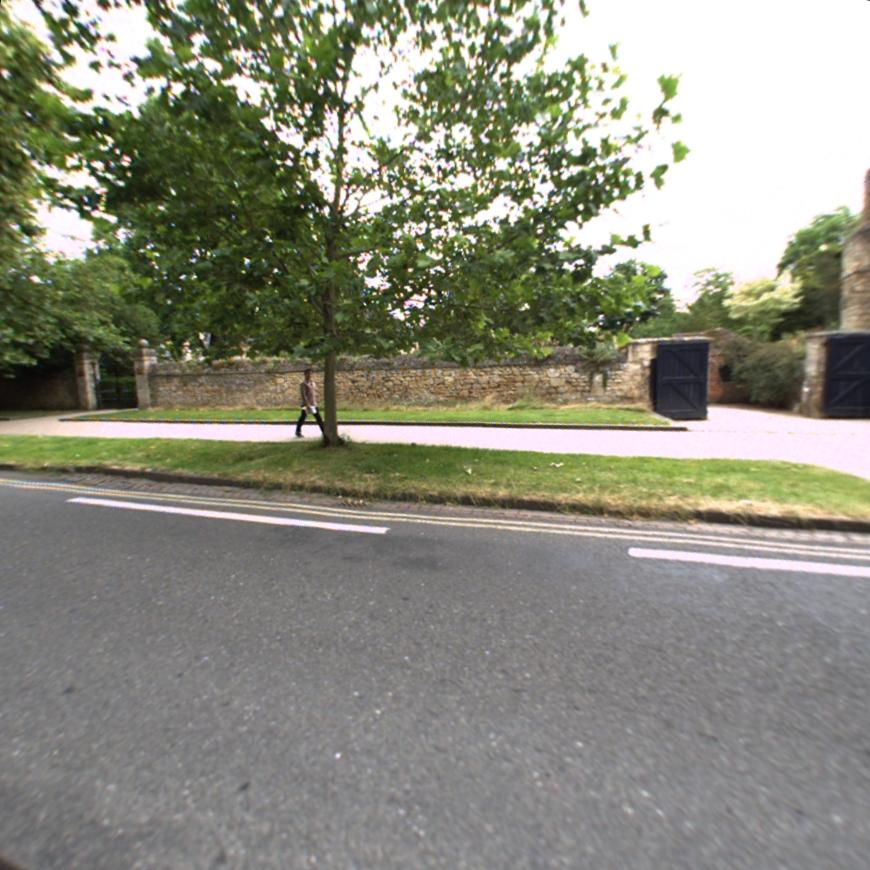
\includegraphics[width=0.19\linewidth]{images/ex_query/dataset4.jpg}
		}
	\end{figure}
	
	\only<1>{Dataset training (green), validation (blue) and testing (red) areas.}
	\only<2>{Examples of queries with corresponding dataset candidates of the testing set.}
\end{frame}

\begin{frame}{Building dense modality map}
	\begin{figure}[t]
			\newcolumntype{Y}{>{\centering\arraybackslash}X}
			\centering
			\begin{footnotesize}
			\begin{tabularx}{\linewidth}{Y Y Y}
				\textbf{Image}	  & \textbf{Points cloud} 			& \uncover<2>{\textbf{Dense depth map}}
			\end{tabularx}
			\end{footnotesize}
			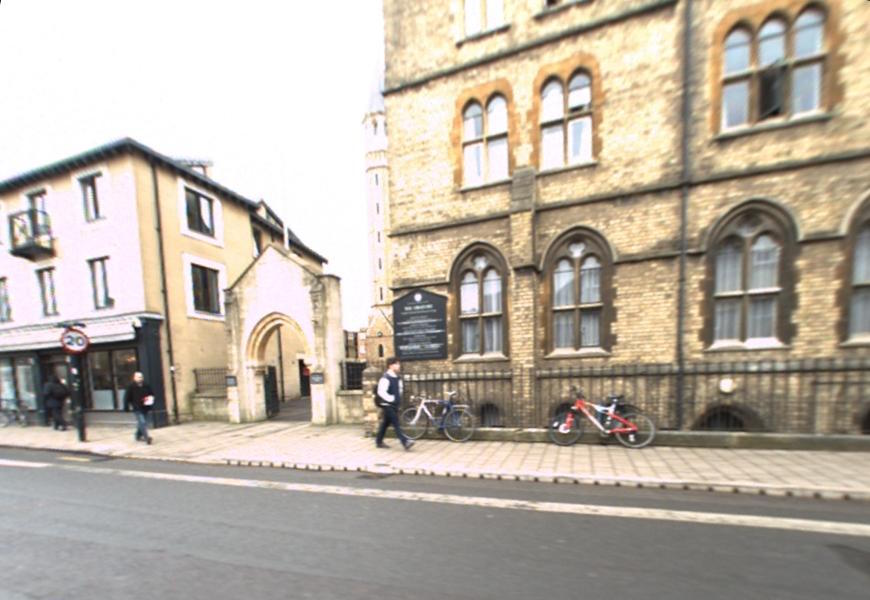
\includegraphics[width=0.33\linewidth]{images/dense_map_creation/image0.jpg}\hfill
			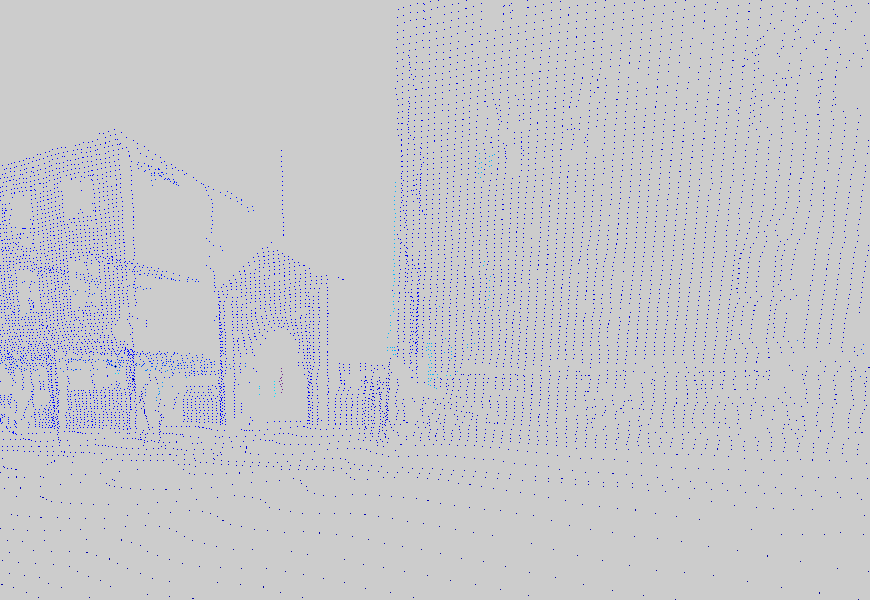
\includegraphics[width=0.33\linewidth]{images/dense_map_creation/sparsedepth0.png}\hfill
			\uncover<2>{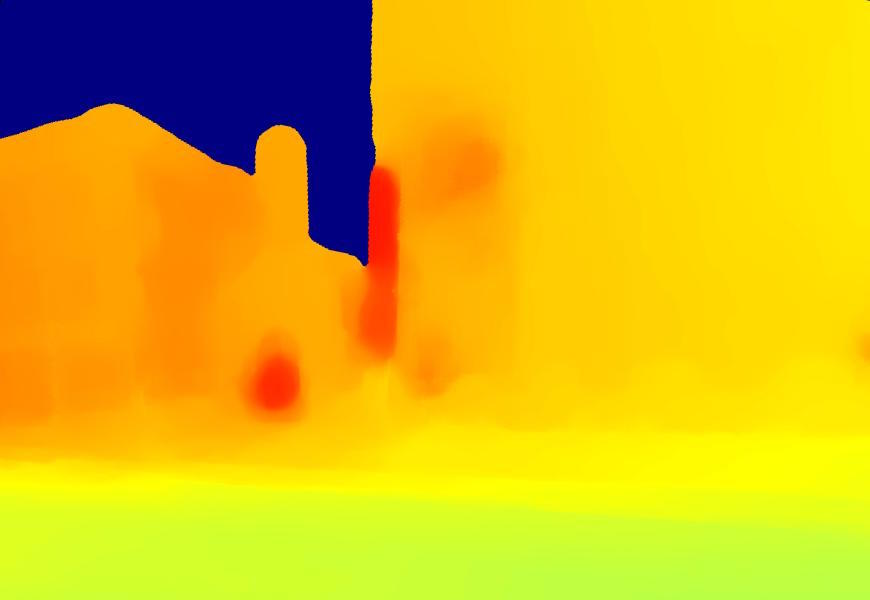
\includegraphics[width=0.33\linewidth]{images/dense_map_creation/densedepth0.jpg}}\hfill
			
			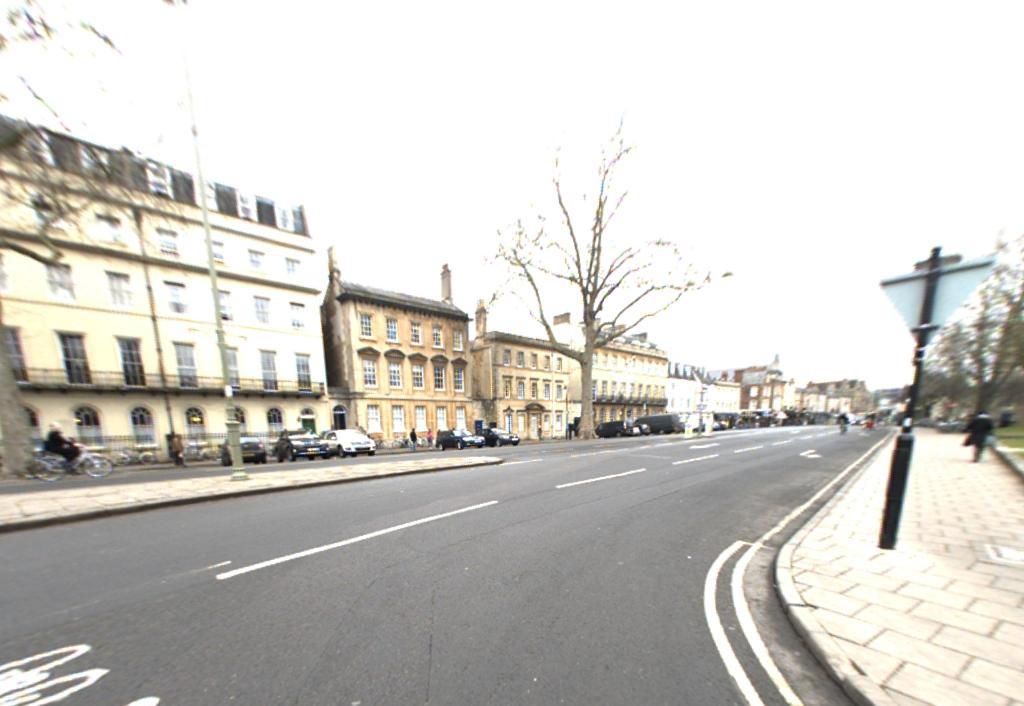
\includegraphics[width=0.33\linewidth]{images/dense_map_creation/image1.jpg}\hfill
			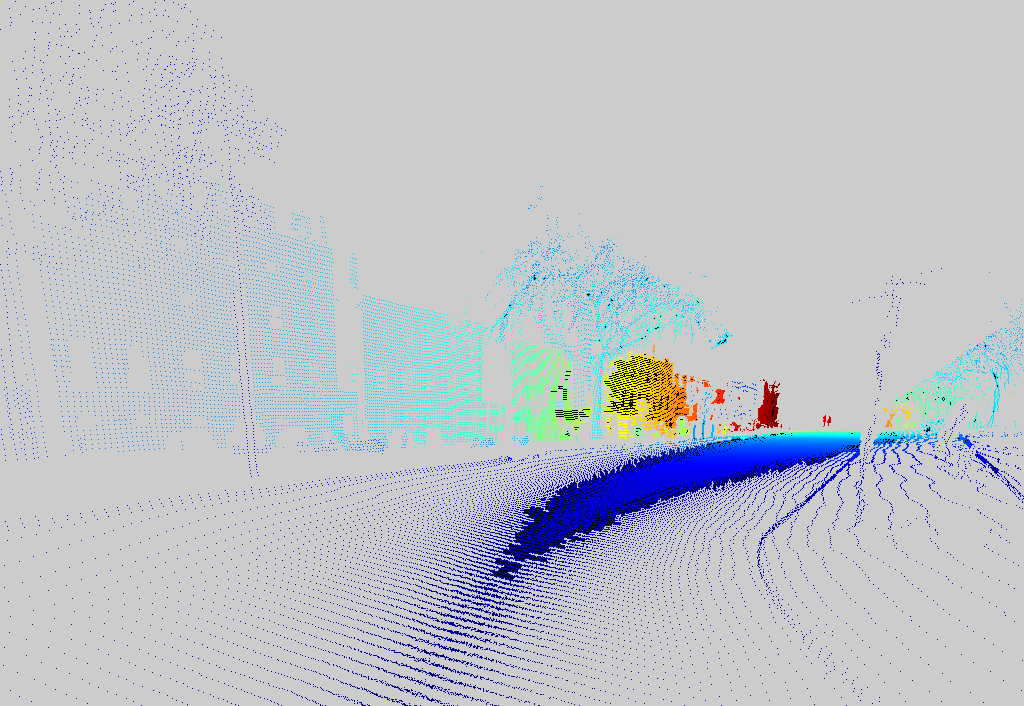
\includegraphics[width=0.33\linewidth]{images/dense_map_creation/sparsedepth1.png}\hfill
			\uncover<2>{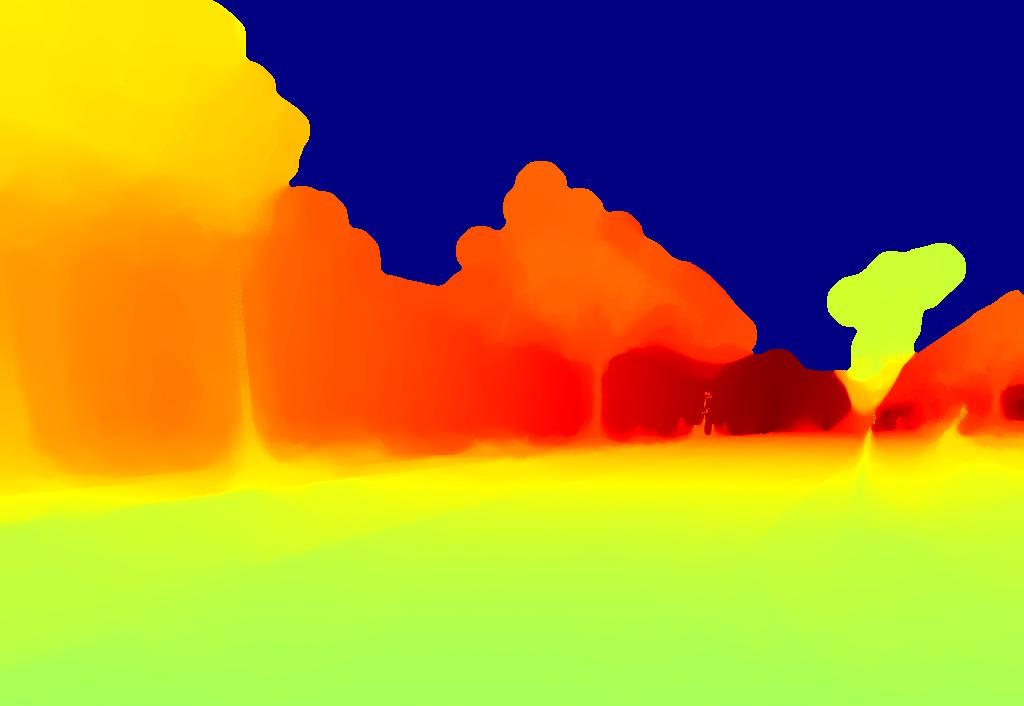
\includegraphics[width=0.33\linewidth]{images/dense_map_creation/densedepth1.jpg}}\hfill
	\end{figure}
	
	We use the algorithm proposed in~\cite{Bevilacqua2017} to create a dense modality map from an image and the associated point cloud.
\end{frame}

\begin{frame}{Results}
	\begin{figure}[t]
		\centering
		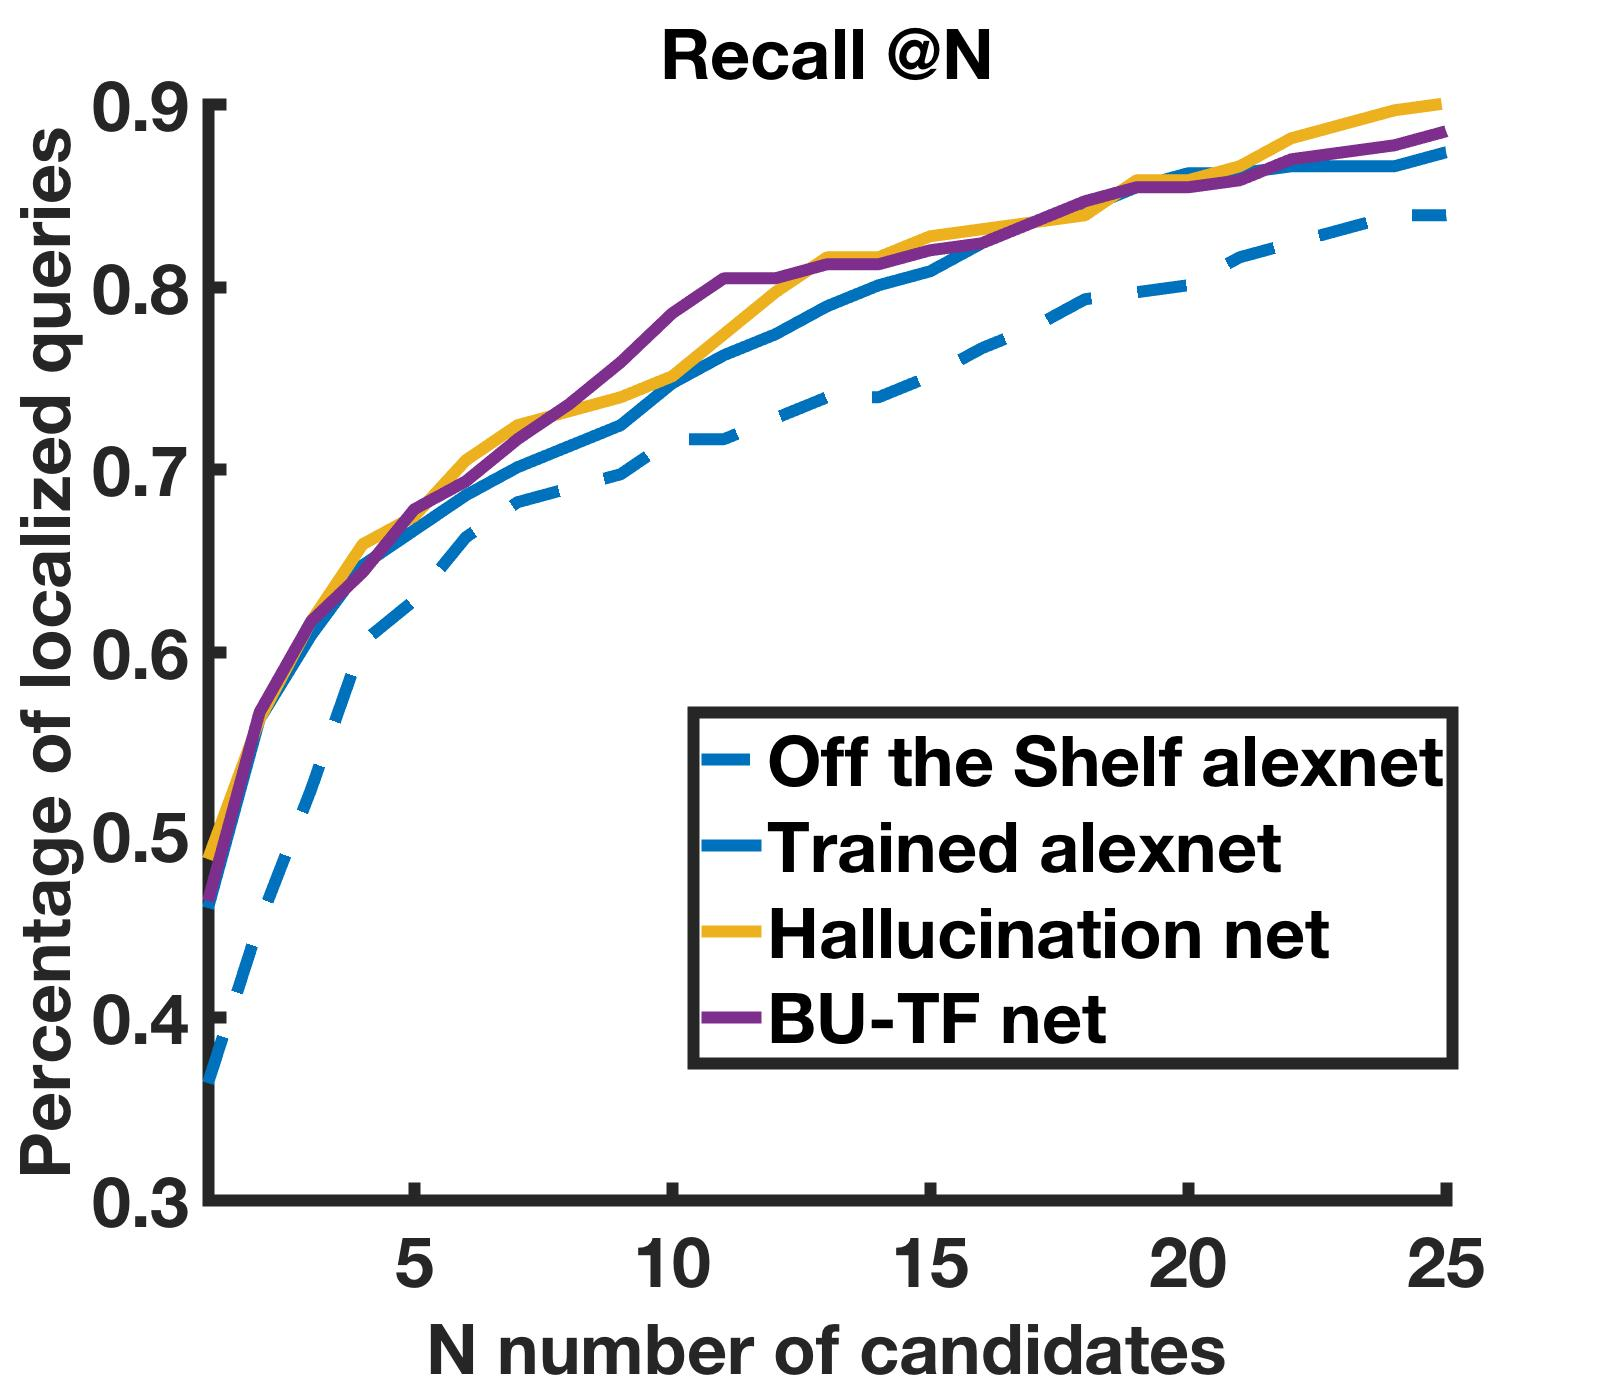
\includegraphics[width=0.499\linewidth]{images/global_res/recall.jpg}\hfill
		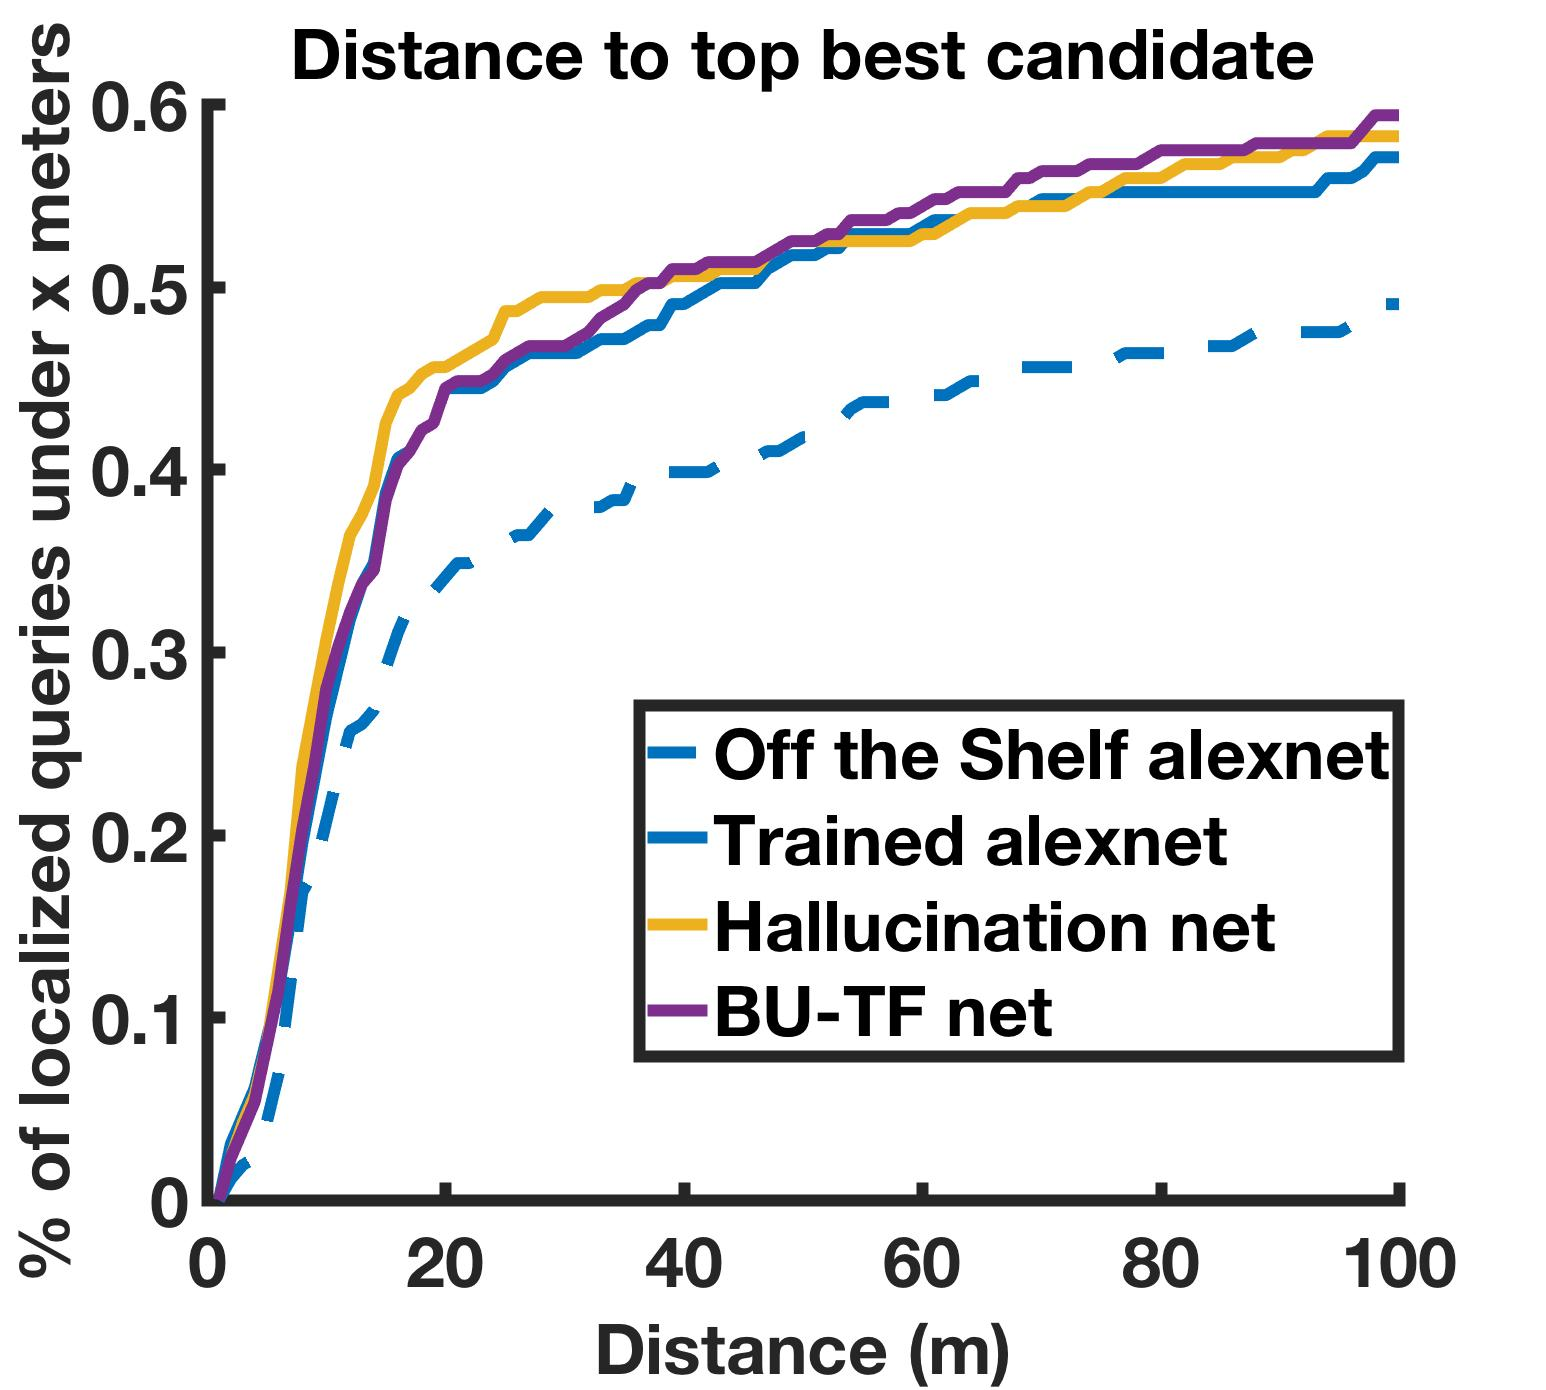
\includegraphics[width=0.499\linewidth]{images/global_res/dist.jpg}			
	\end{figure}	
	Off-the-shelf: network only trained on ImageNet, no fine-tuning for this specific task and on these specific data.
\end{frame}

\begin{frame}{Results - Diversification loss}
	\begin{figure}[t]
		\centering
		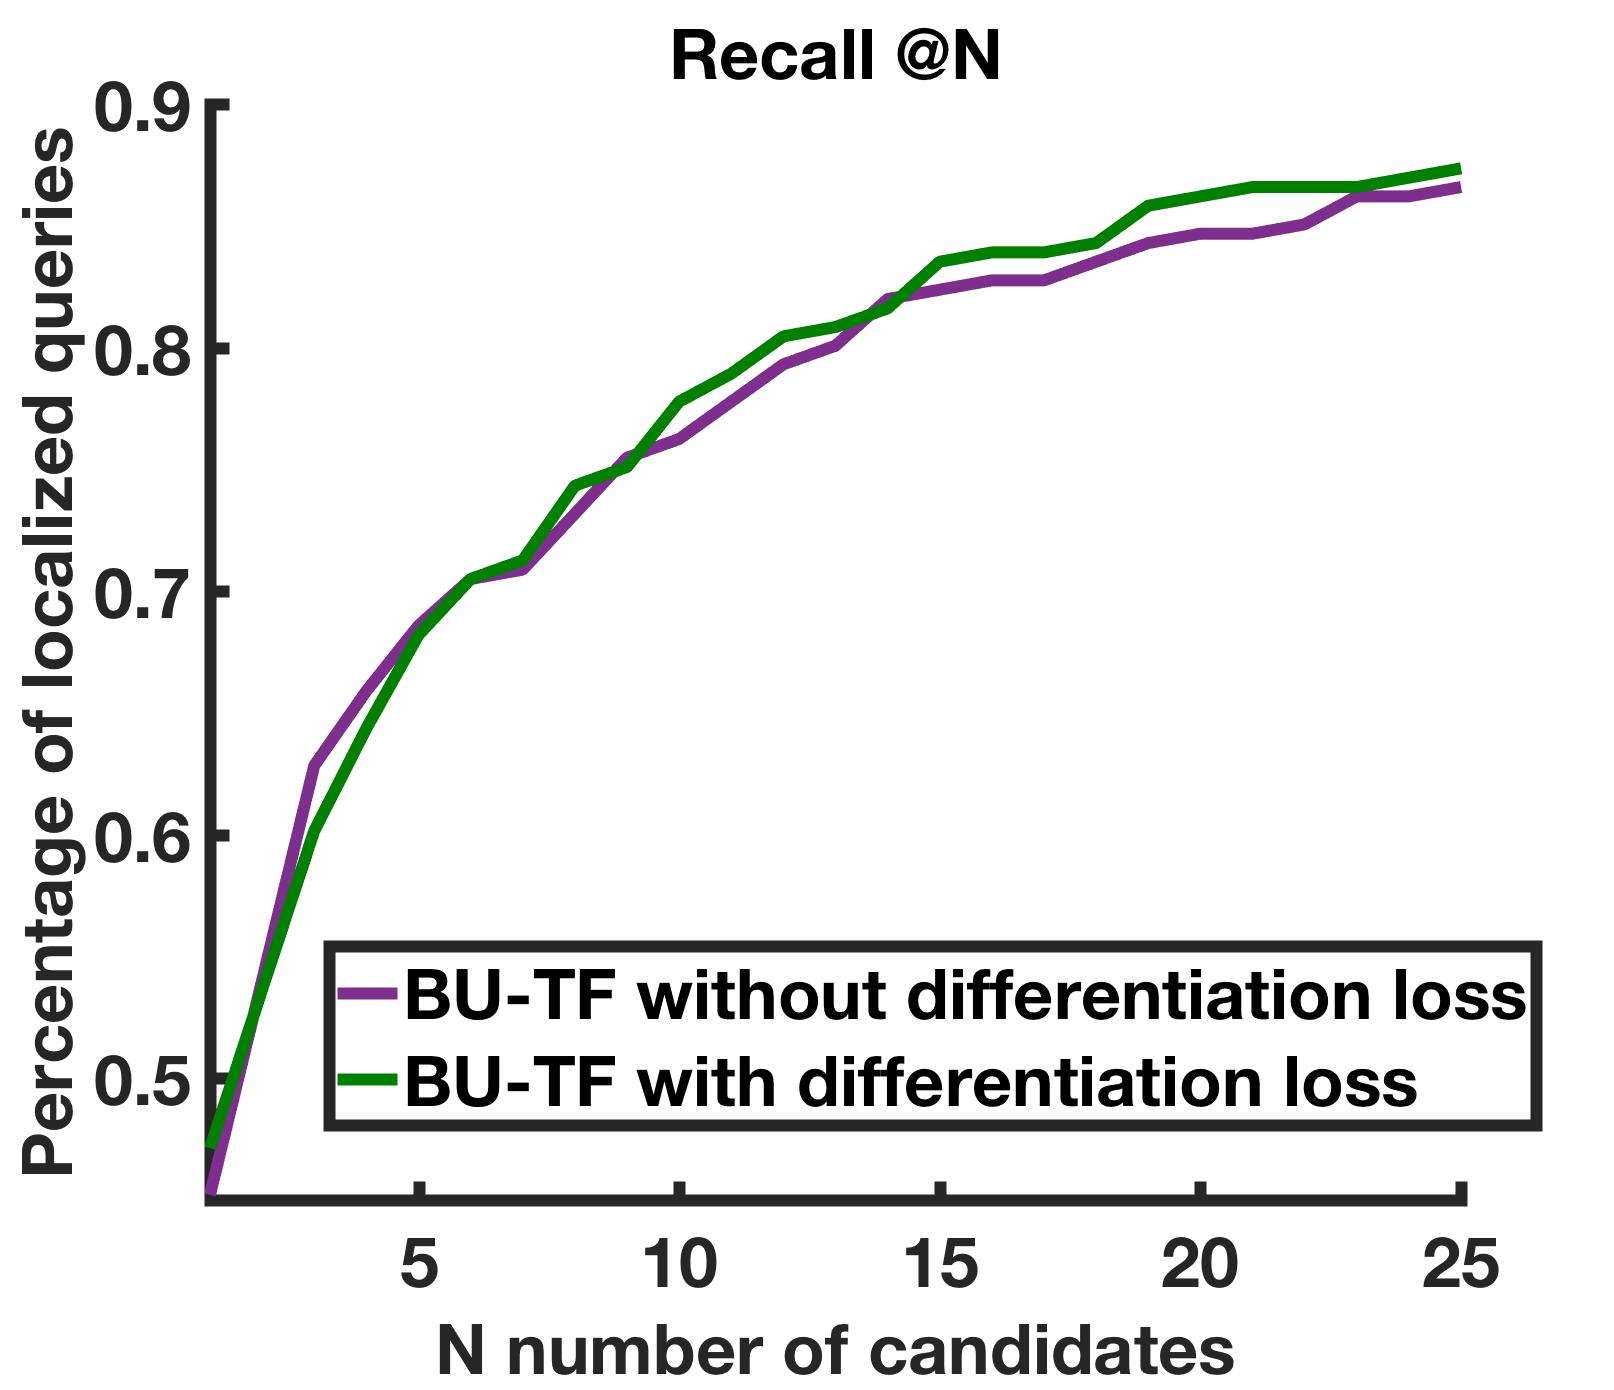
\includegraphics[width=0.499\linewidth]{images/diffloss_res/recall.jpg}\hfill
		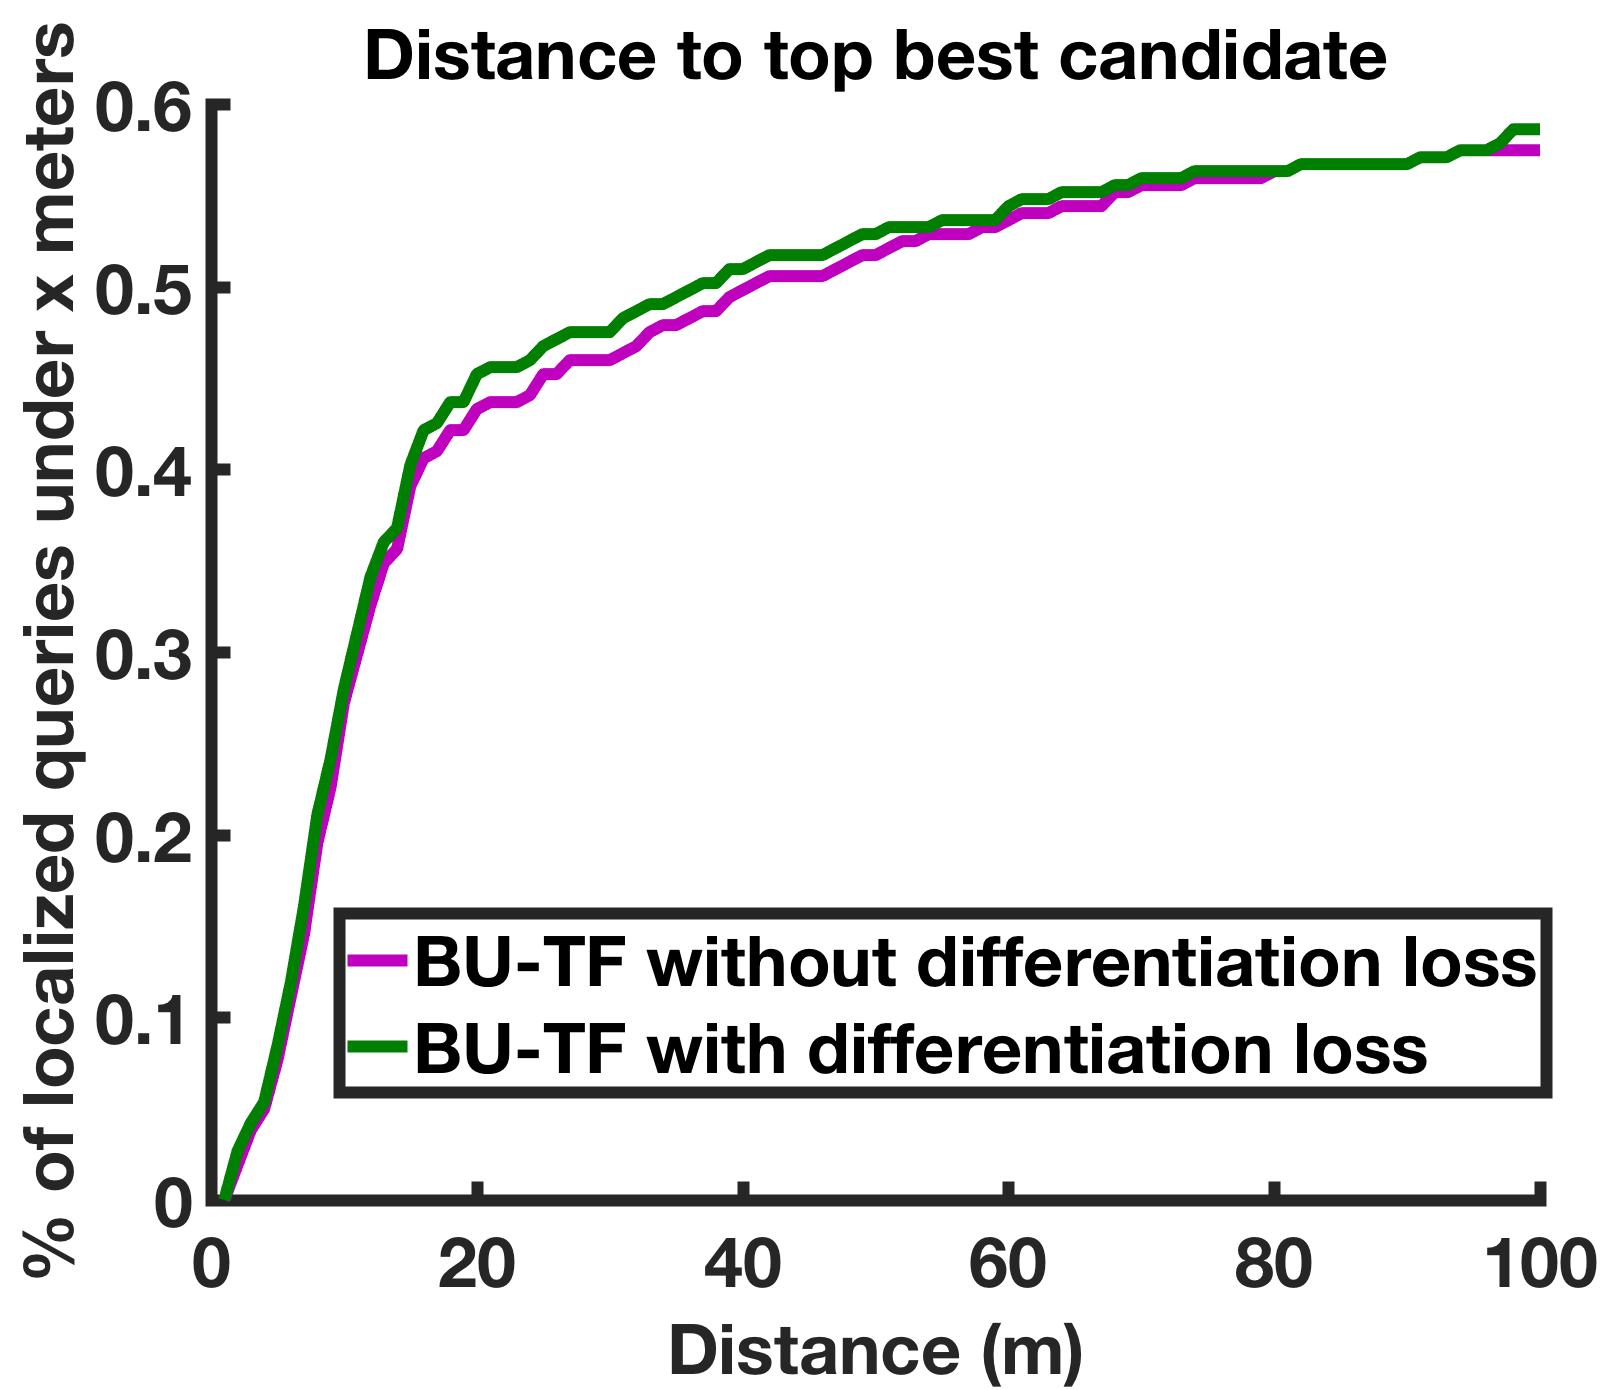
\includegraphics[width=0.499\linewidth]{images/diffloss_res/dist.jpg}
	\end{figure}	
\end{frame}

\begin{frame}{Results - Visual inspection}
	\begin{minipage}[c][0.65\textheight]{0.19\linewidth}
		Main modality 
		\vspace{1.5cm}		
		
		Side modality
		\vspace{1.5cm}
		
		Reconstructed side modality
	\end{minipage}\hfill
	\begin{minipage}[c][0.7\textheight]{0.75\linewidth}
		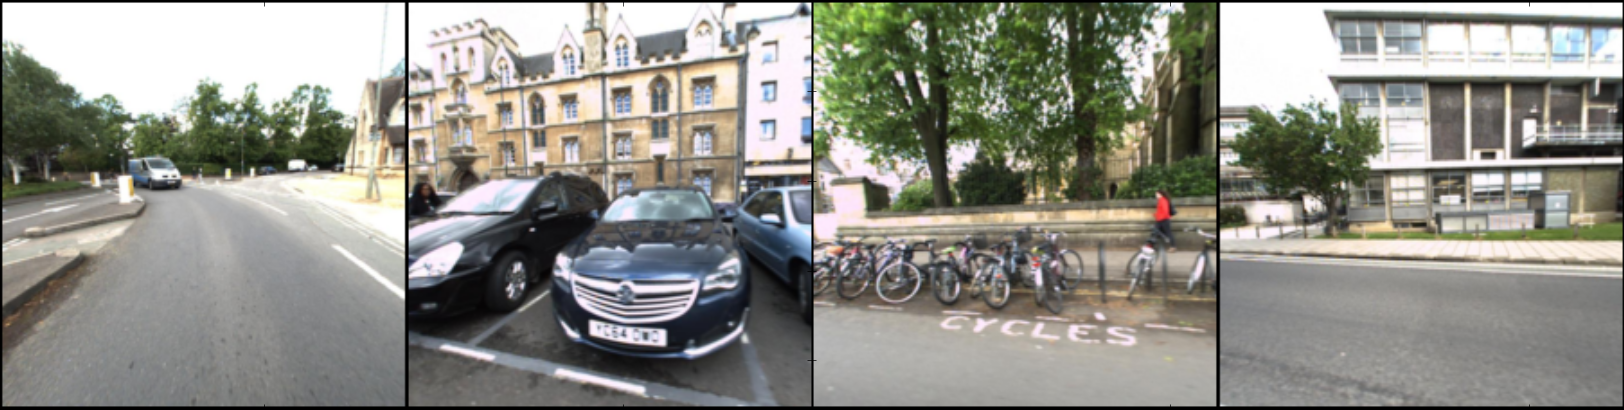
\includegraphics[width=0.95\linewidth]{images/visual_results/mod_rgb.png}
		\vfill		
		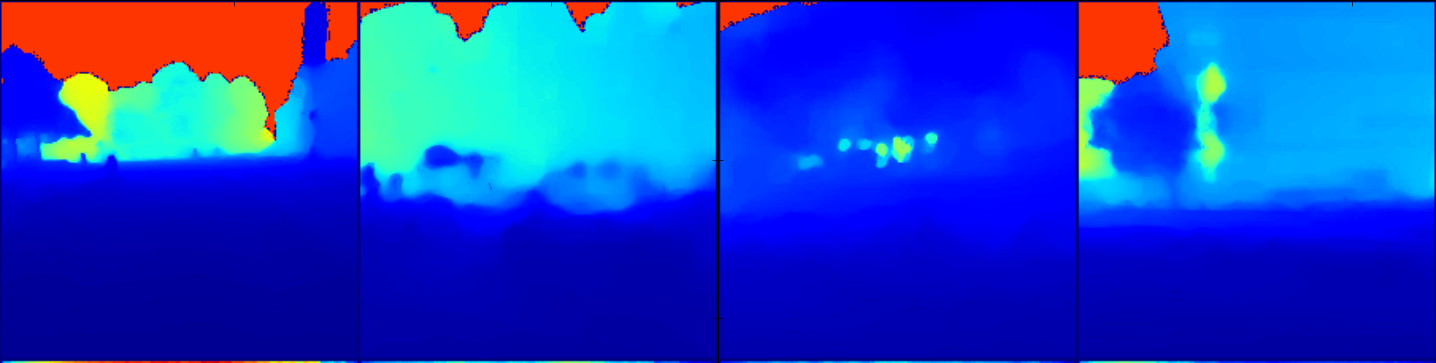
\includegraphics[width=0.95\linewidth]{images/visual_results/gt_depth.png}
		\vfill		
		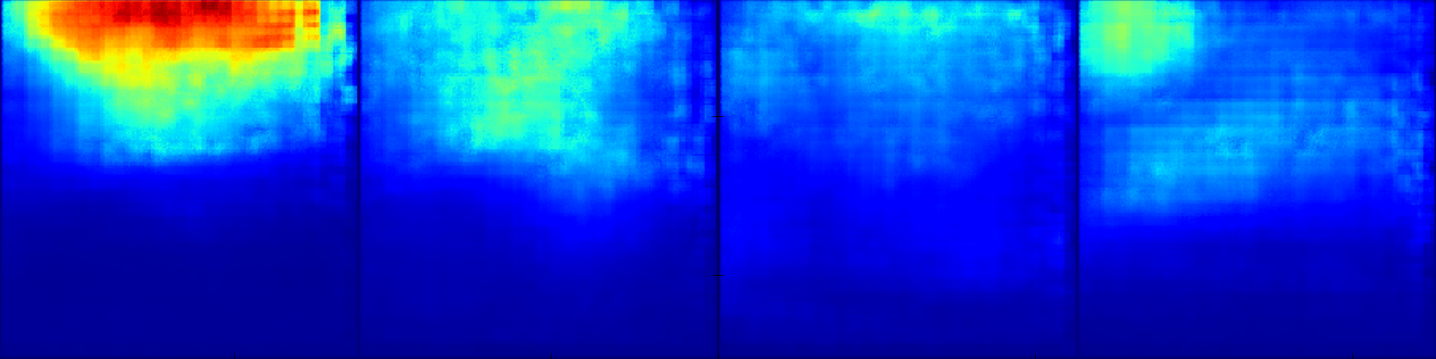
\includegraphics[width=0.95\linewidth]{images/visual_results/reconstructed_maps.png}
	\end{minipage}	
\end{frame}
